\section{Mô phỏng mạch trên PSpice}
\subsection{Mạch 3.3V regulator}
Chúng ta sẽ sử dụng đầu vào là nguồn DC 20 V để kiểm thử đầu ra.

\begin{figure}[ht]
    \centering
    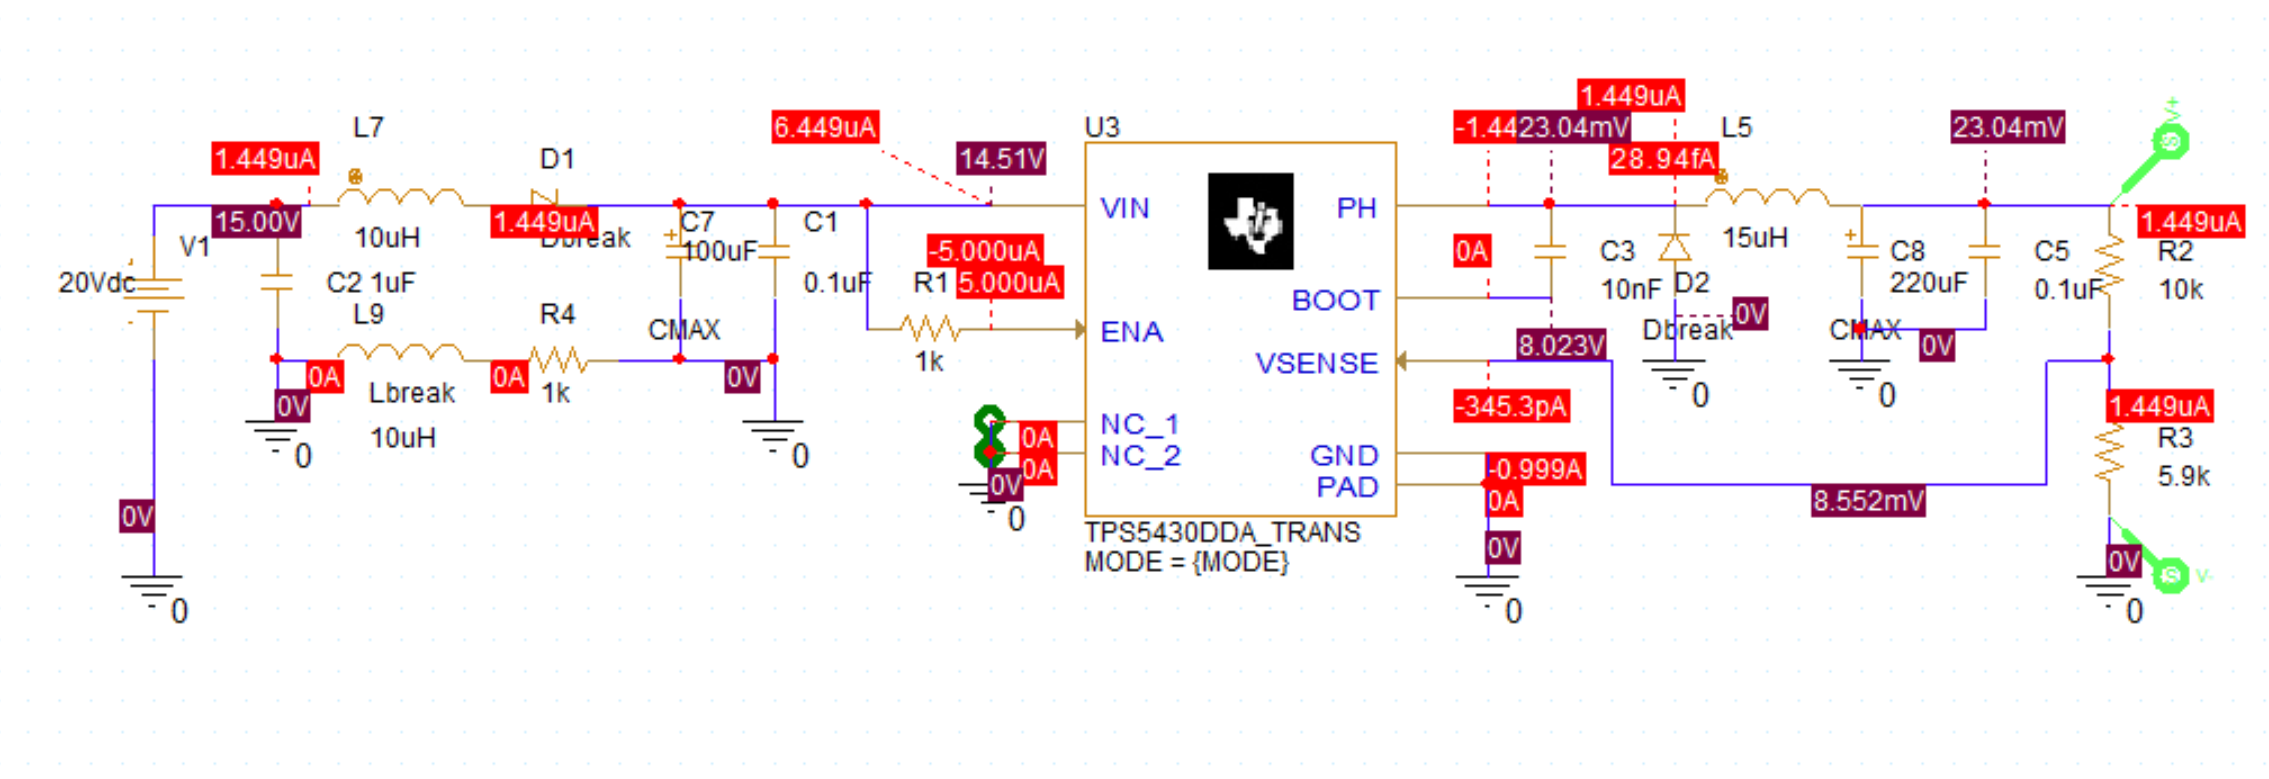
\includegraphics[width=1\textwidth]{graphics/section4/f1.png}
    \caption{Nguồn DC 20 V}
\end{figure}

\textbf{Ảnh mô phỏng}
\begin{figure}[ht]
    \centering
    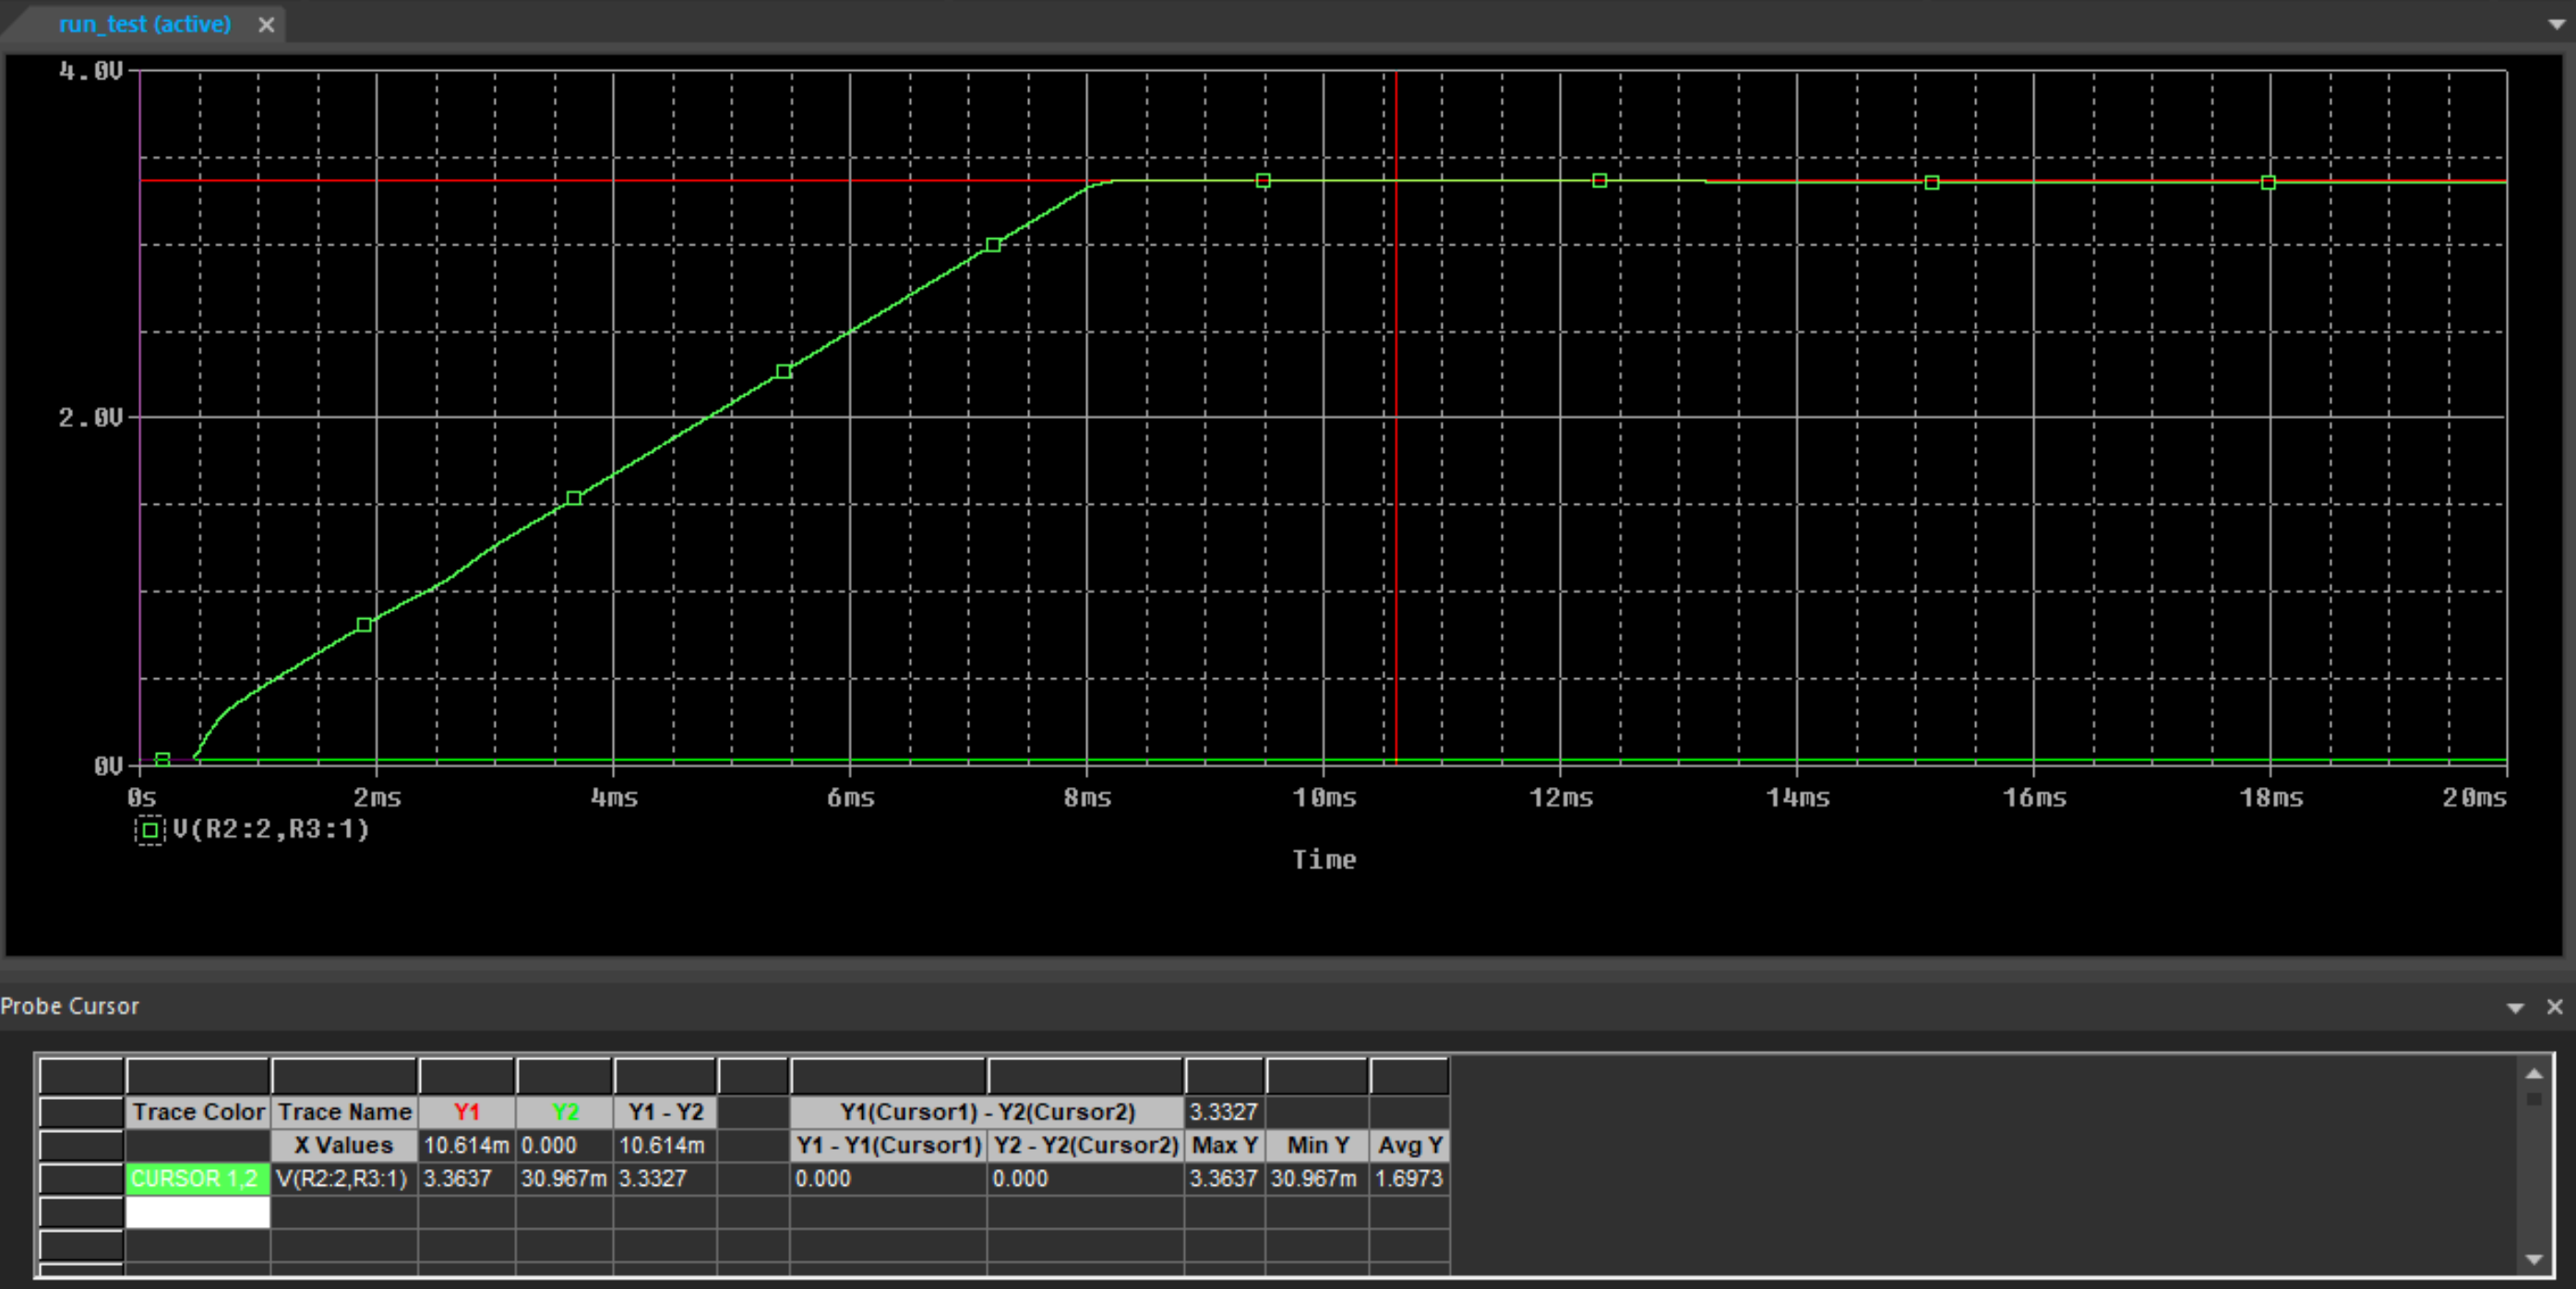
\includegraphics[width=1\textwidth]{graphics/section4/f2.png}
    \caption{Nguồn DC 20 V}
\end{figure}

\textbf{Nhận xét: }Nguồn đầu vào 20 V DC khi qua mạch cho đầu ra lúc đầu điện áp tăng dần từ 0 V và ổn định ở mức 3.3V DC. Như vậy, mạch đã đáp ứng yêu cầu cung cấp nguồn đầu vào ổn định ở mức điện áp 3.3 V cho bo vi điều khiển ESP32 wroom 32 từ nguồn điện.  

\pagebreak
\subsection{Current sensor circuit}
Current sensor TA12 và TA17 là những cảm biến để đo dòng điện AC tối đa 5A với TA12 và dòng tối đa 10A với TA17. Đầu ra của 2 cảm biến là tín hiệu dòng AC có cùng tần số với dòng đang đo và biên độ nhỏ hơn. Khi có đo dòng điện, cảm biến sẽ tạo dòng điện AC vào mạch sẽ được đệm và lọc thông thấp qua U3A vào chân ADC1\_CH6 về vi điều điều khiển ESP32 wroom 32 để đo đạc giá trị.

Nhưng trong mô phỏng này, ta sẽ dùng cảm biến dòng khác là TMCS1108 để thay thế cho TA12 và TA17 để kiểm thử chức năng đệm điện áp (buffer) và bộ lọc thông thấp (low pass filter) của mạch dùng opamp này.

TMCS1108A3U là mã của một loại cảm biến dòng điện (current sensor) sử dụng hiệu ứng Hall. Đây là cảm biến dòng điện không tiếp xúc Có khả năng đo dòng điện cả dòng một chiều (DC) và dòng xoay chiều (AC), dải đo rộng, phù hợp với nhiều ứng dụng khác nhau (lên đến 7.25 A với nguồn cấp cho nó là 3.3V).

Đầu ra của TMCS1108A3U là điện áp phụ thuộc vào dòng điện cần đo, $V_{out} = V_{offset} + GAIN.I$
Với \begin{itemize}
    \item GAIN = Hệ số khuếch đại hoặc độ nhạy của cảm biến (mV/A). Với TMCS1108A3U, thì GAIN = 200 mV/A.
    \item $V_{out}$: Điện áp đầu ra của cảm biến.
    \item Voffset: Điện áp tại 0A (thường là 2.5V cho các cảm biến đo cả AC và DC).
\end{itemize}

Như vậy, dựa vào tham chiếu giá trị điện áp của ADC1\_CH7 qua opamp U3B và điện áp của ADC1\_CH6 để tính toán đo lường dòng điện.\

\textbf{Mô phỏng:} điện áp của ADC1\_CH7 và ADC1\_CH6 khi dùng TMCS1108A3U để đo dòng điện AC với tần số là 1000 Hz và biên độ $I = \dfrac{220}{1000} = 0.22 A$.
 \pagebreak
\begin{figure}[ht]
    \centering
    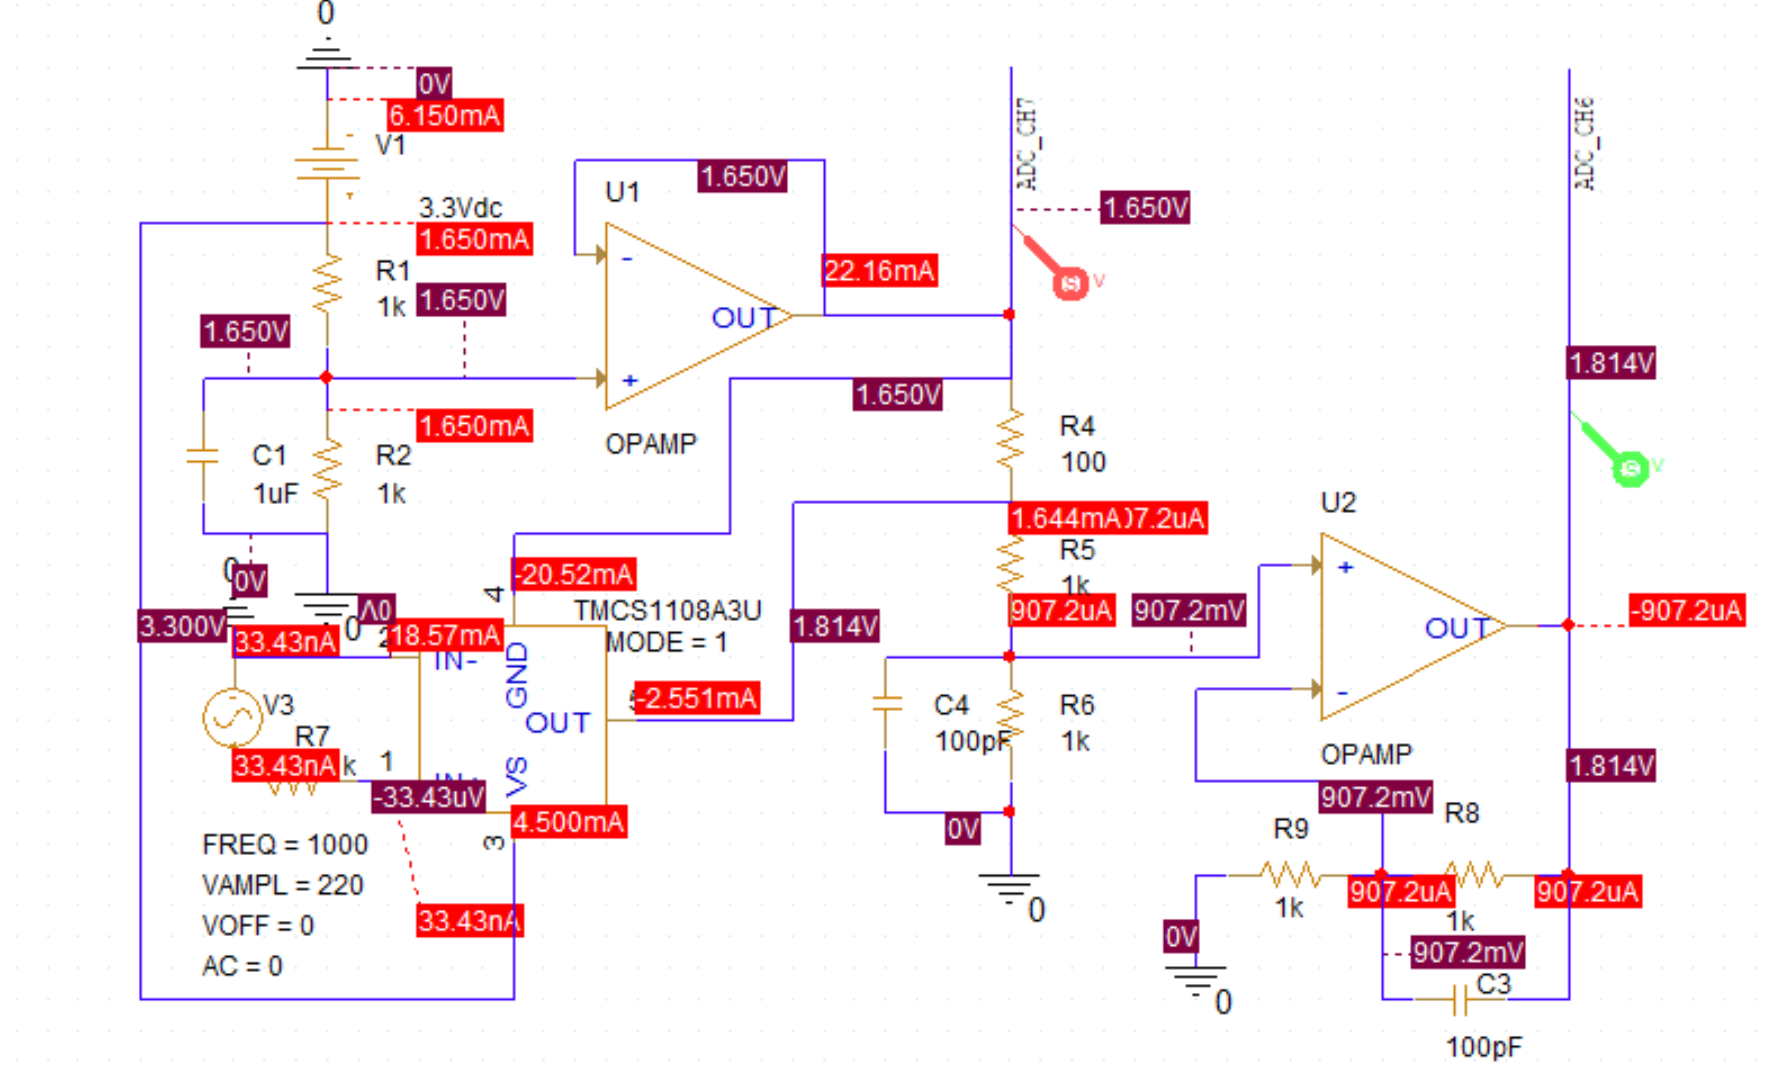
\includegraphics[width=0.8\textwidth]{graphics/section4/f21.png}
    \caption{Đo nguồn AC}
\end{figure}

\begin{figure}[ht]
    \centering
    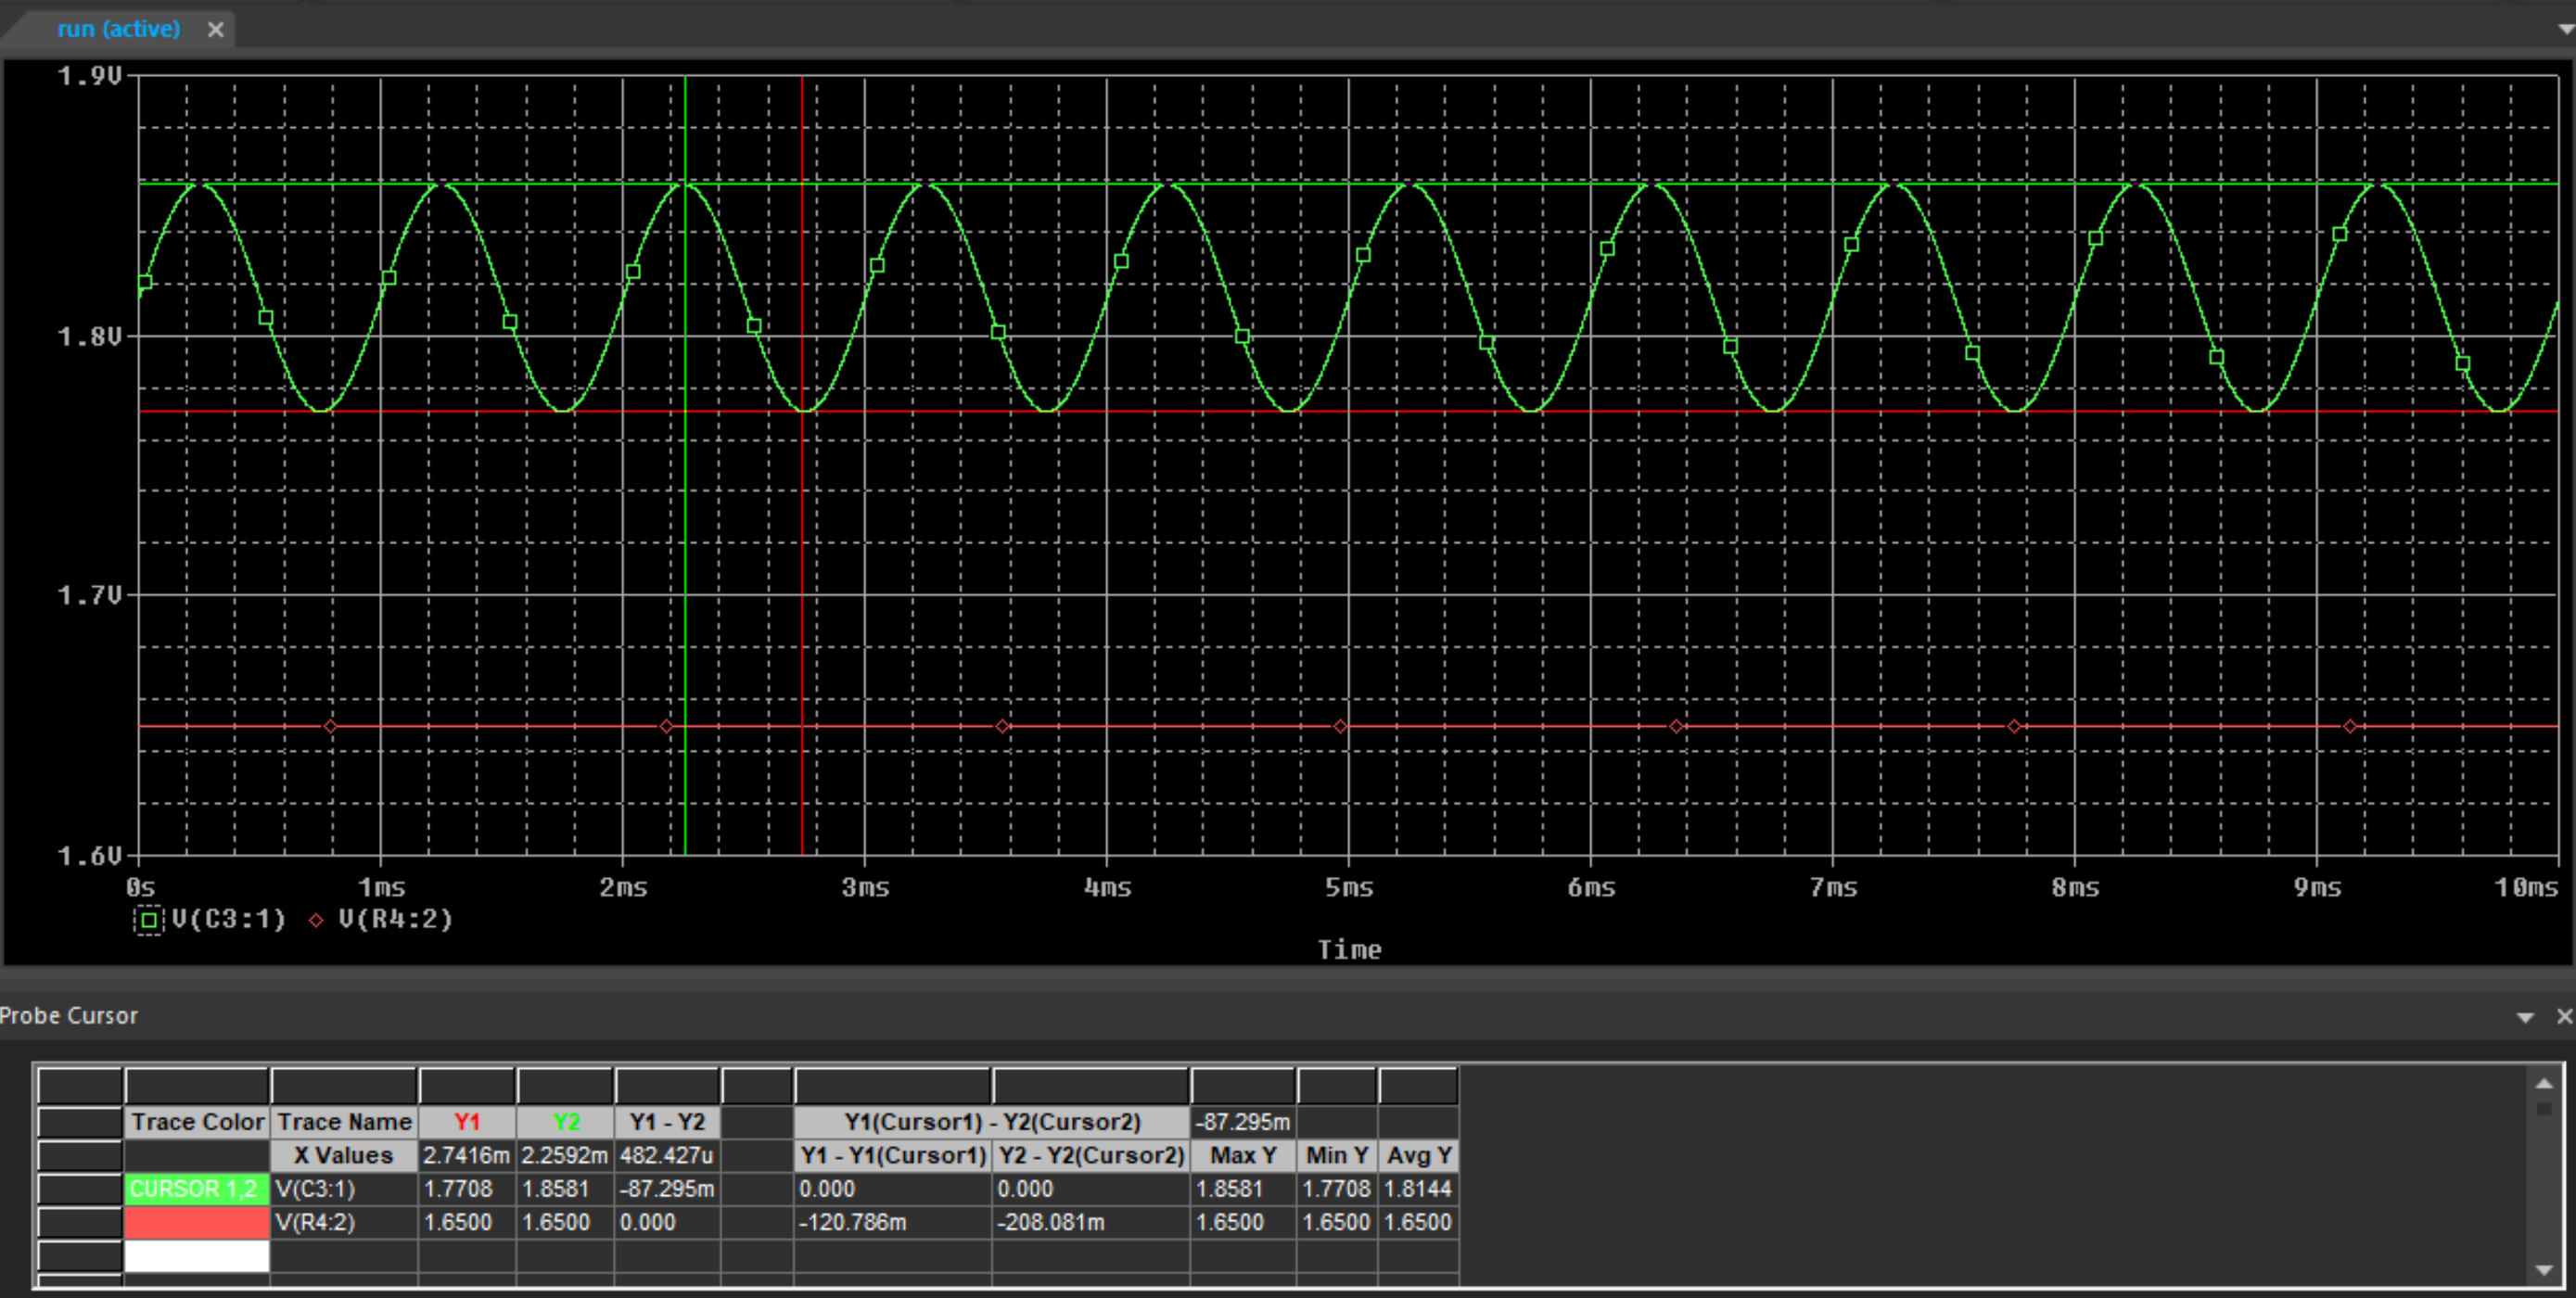
\includegraphics[width=0.8\textwidth]{graphics/section4/f22.png}
    \caption{Đo nguồn AC}
\end{figure}
\pagebreak

\textbf{Nhận xét:} Ta thấy đầu ra của ADC\_CH6 được opamp khếch đại lên Gain = 2, điện áp tại ADC1\_CH7 cố định ở mức 1.65 V (loại bỏ R6 để tại U3B để tham chiếu trực tiếp điện áp 3.3V/2). Từ đó tính toán để đo lường I của dòng điện cần đo qua $V_{out} = V_{offset} + GAIN.I$.

Tiếp theo, ta sẽ đo dòng điện AC thay đổi tần số để kiểm thử bộ lọc thông áp của mạch tại U3A.

\begin{figure}[ht]
    \centering
    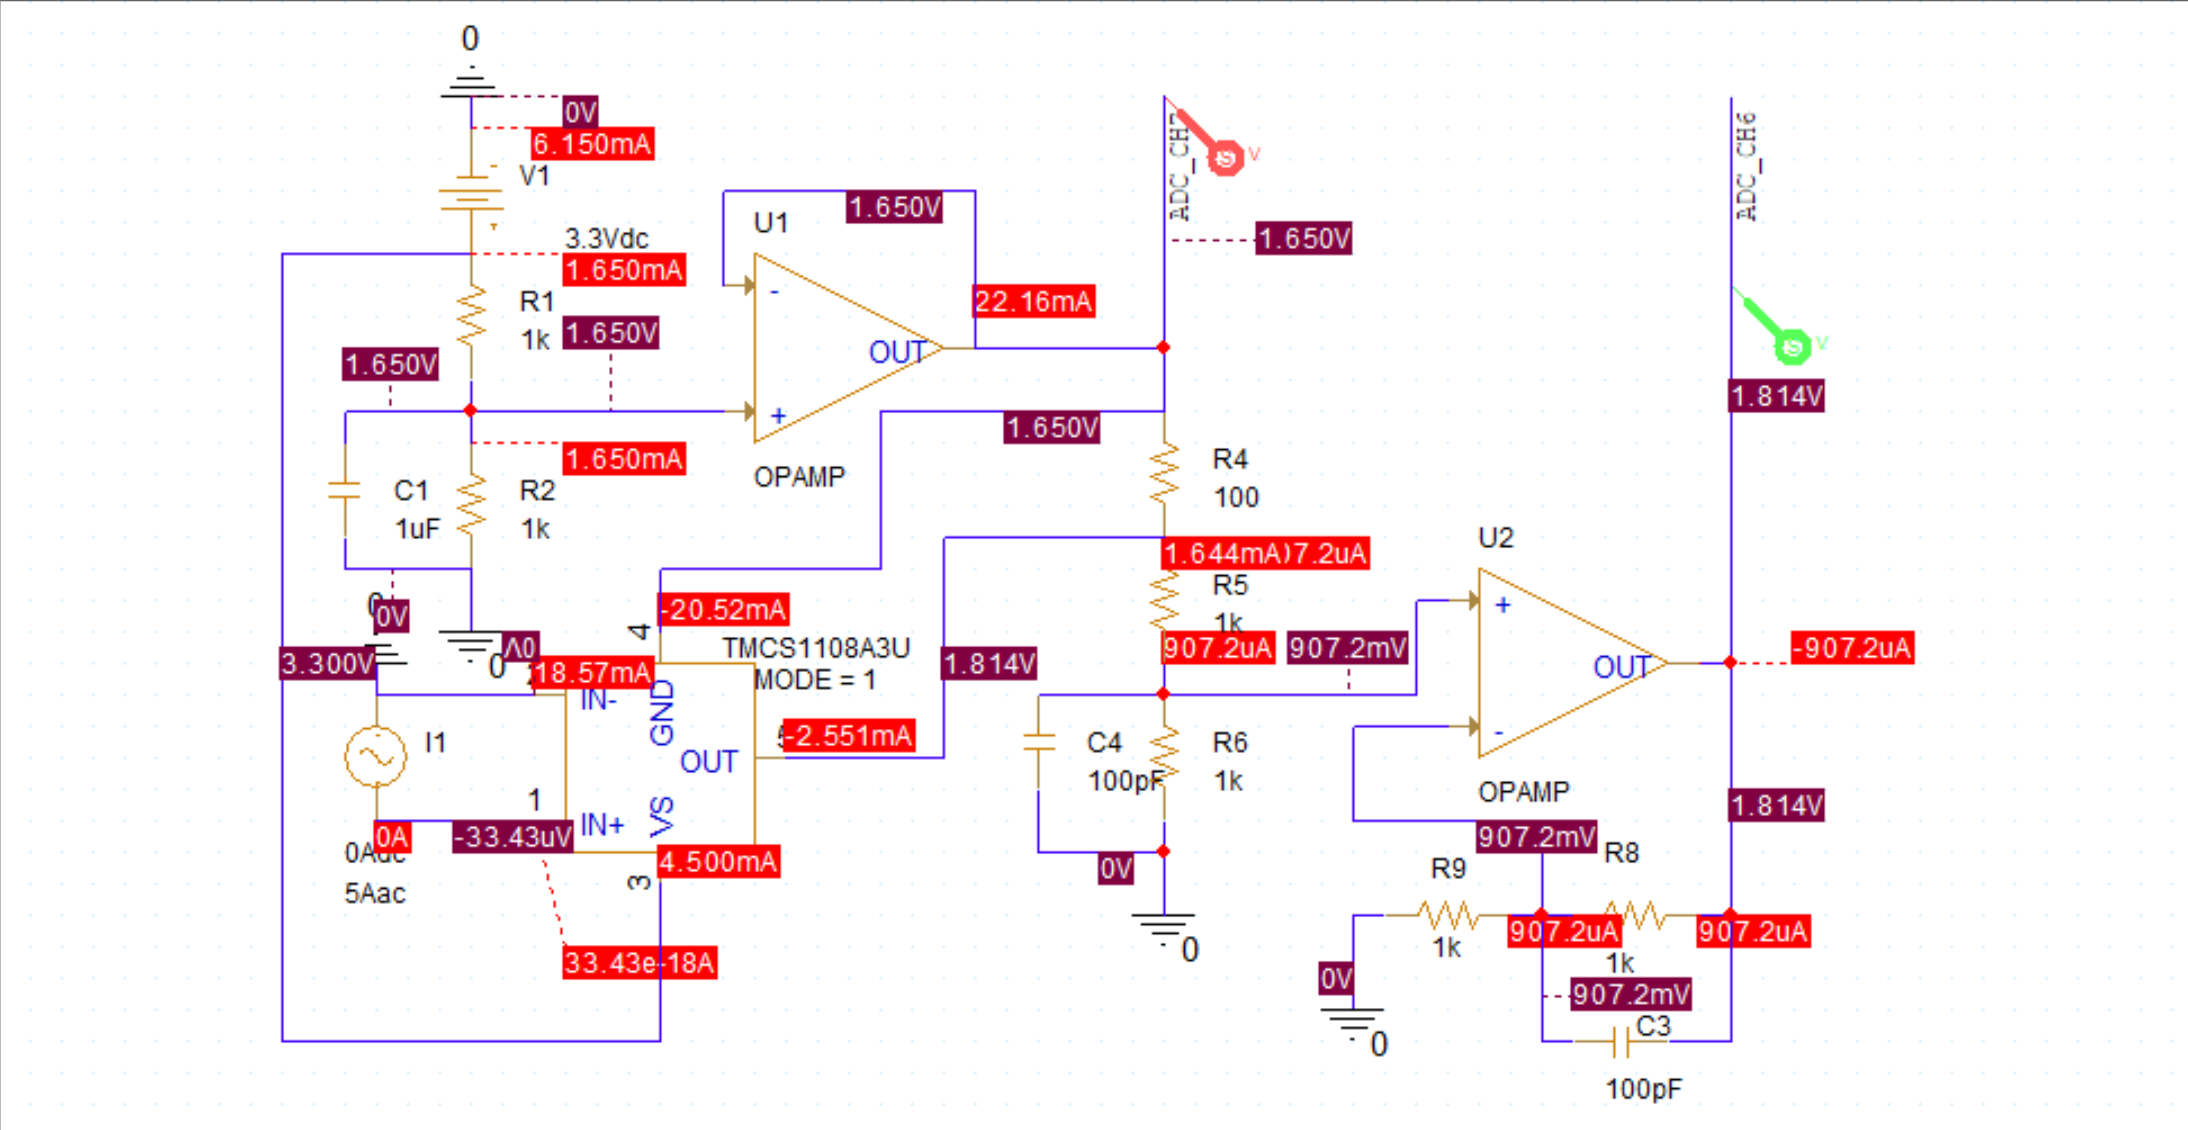
\includegraphics[width=1\textwidth]{graphics/section4/f23.png}
    \caption{Đo nguồn AC}
\end{figure}

\begin{figure}[ht]
    \centering
    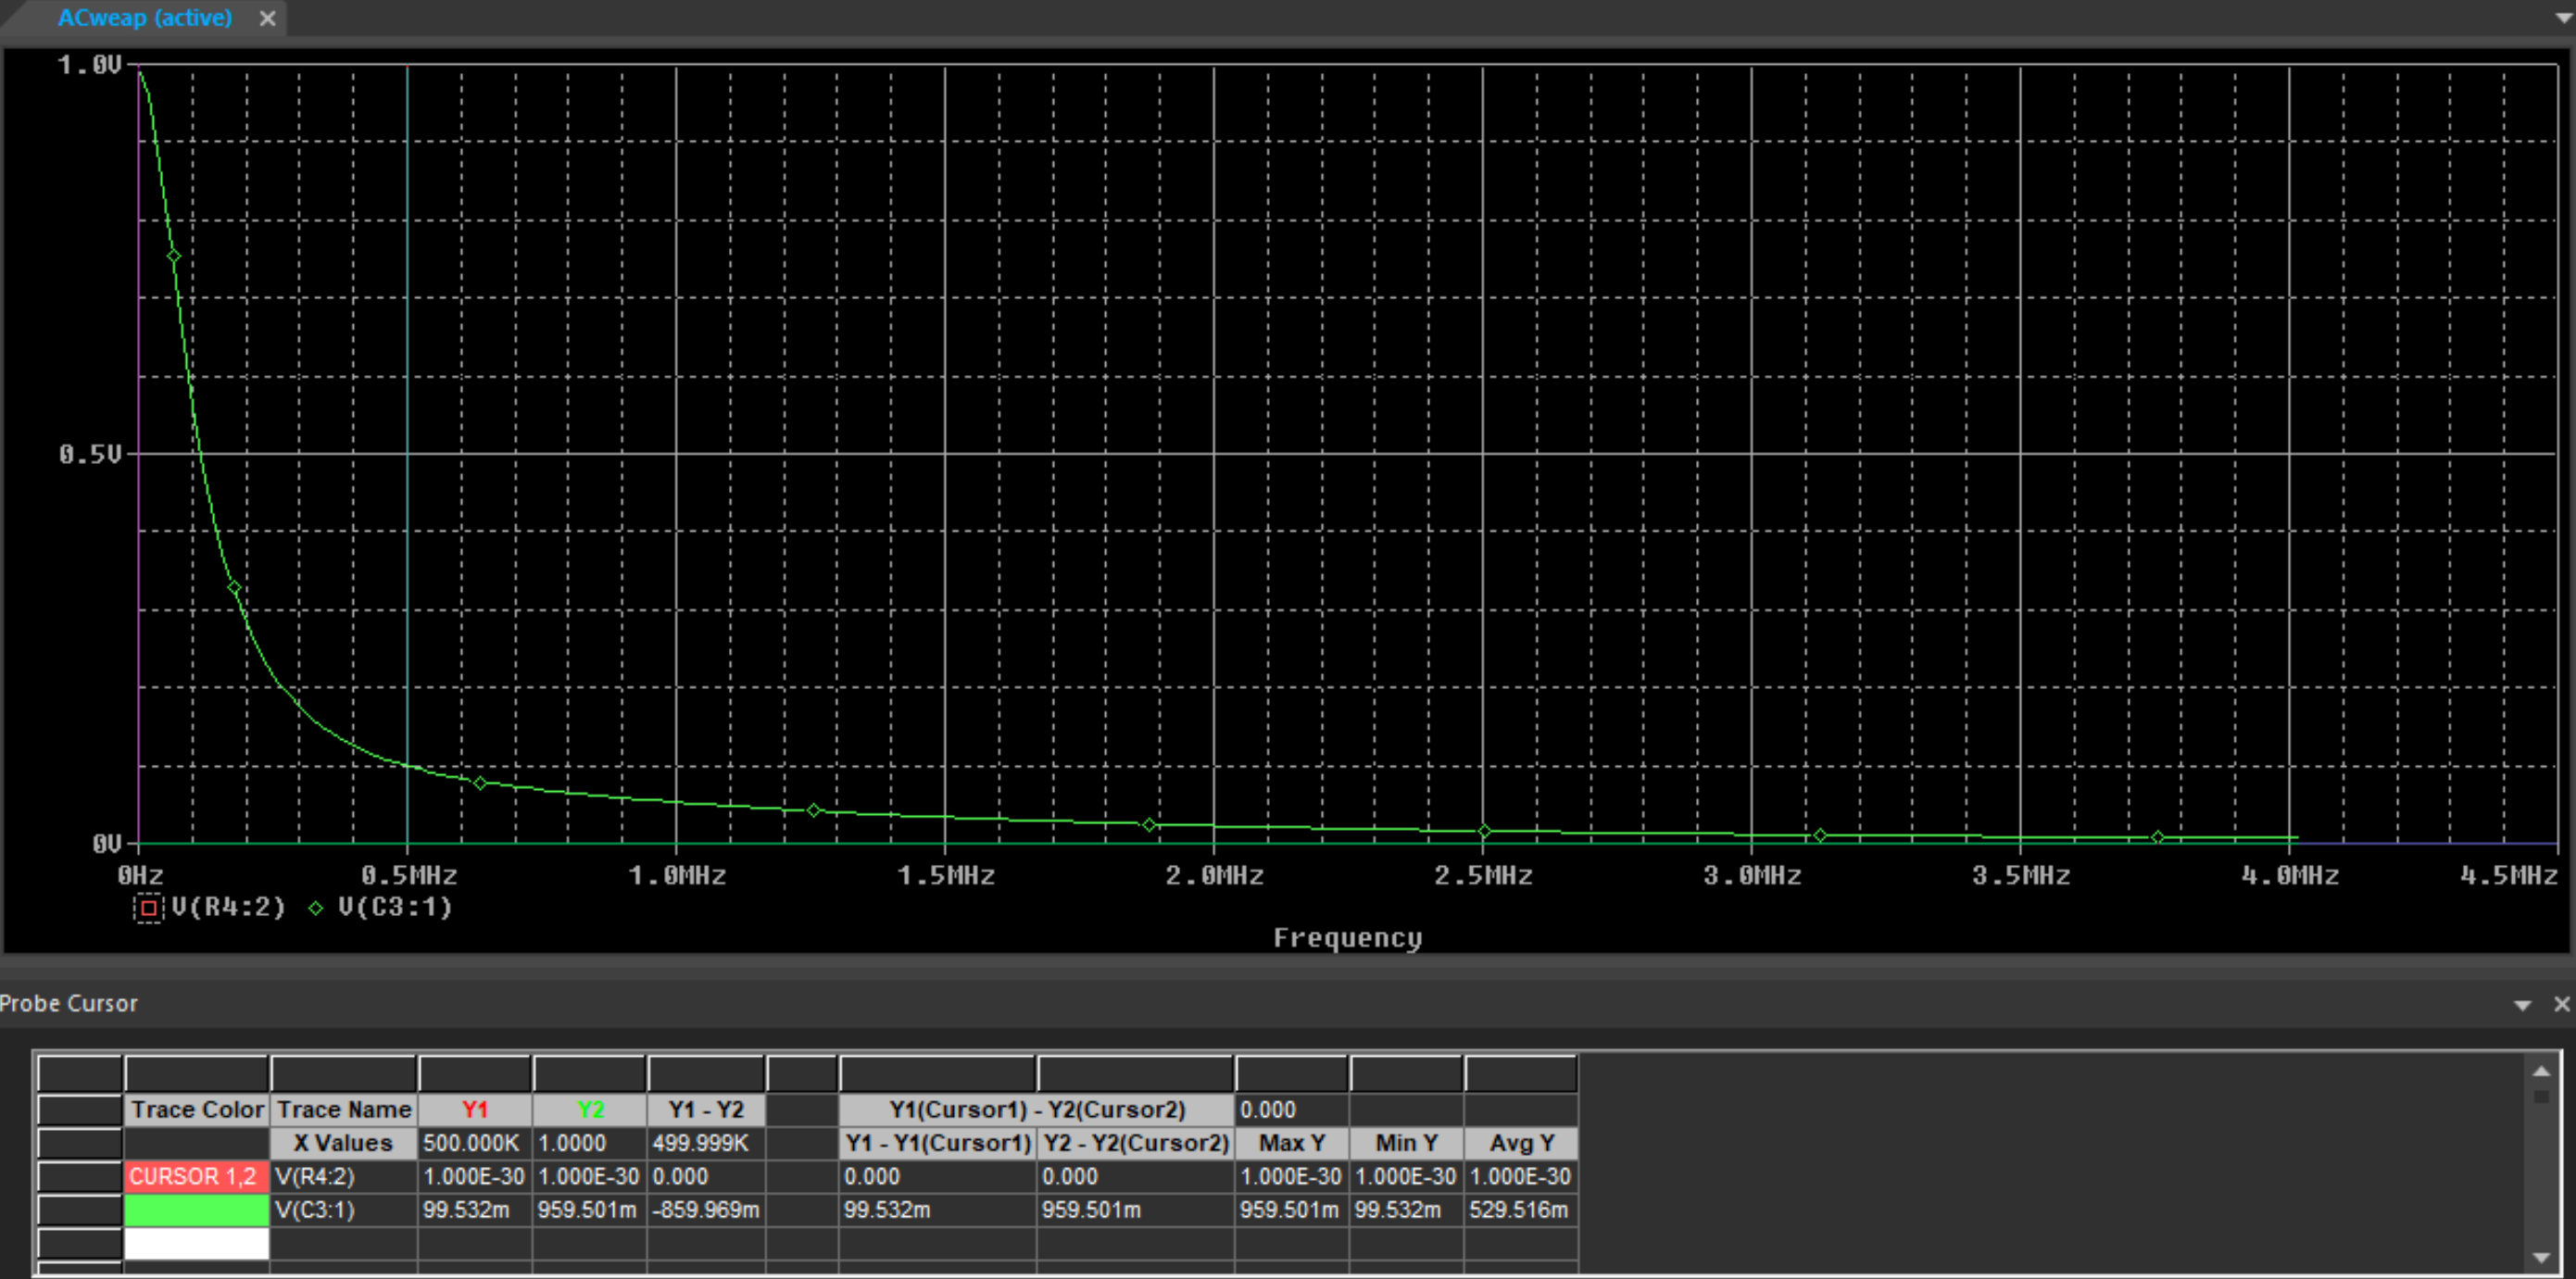
\includegraphics[width=1\textwidth]{graphics/section4/f24.png}
    \caption{Đo nguồn AC}
\end{figure}
\pagebreak

\textbf{Nhận xét:} Ta thấy biên độ AC của ADC1\_CH6 giảm dần khi tần số tăng dần. Điều này cho thấy mạch lọc thông thấp (low pass filter) hoạt động gần đúng với tần số $f_{cutoff} = 1.59 MHz$ tính toán trong phần câu hỏi.


\subsection{Interface with high-current LEDs}

Do điện áp phân cực thuận $V_{f_{RED}} = 1.8V$ tới 2.2V và trong mô phỏng trên PSpice thì $V_F \approx 0.67 V$ nên ta thay bằng 3 diode.
Tương tự, $V_{f_{GREEN}} = 2.8V$ tới 3.2V nên trong mô phỏng ta thay bằng 4 diode.

\pagebreak

\textbf{Mô phỏng}

\begin{figure}[ht]
    \centering
    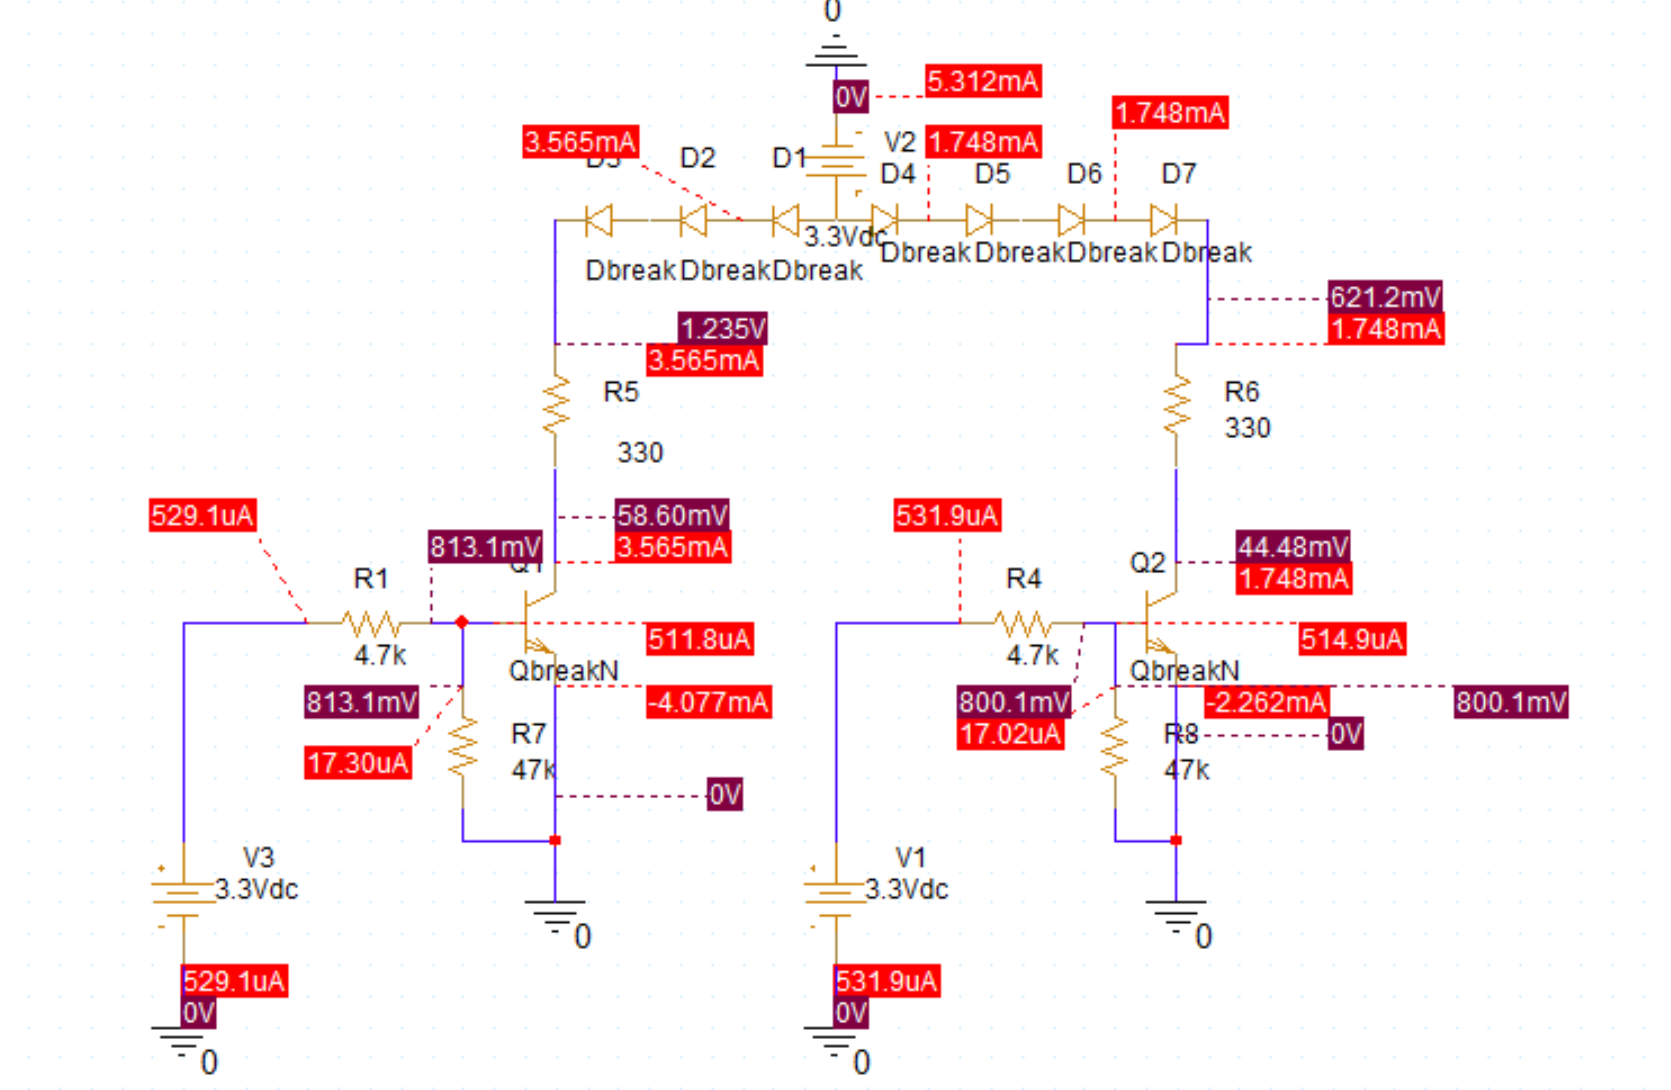
\includegraphics[width=0.95\textwidth]{graphics/section4/f5.png}
    \caption{Simulation 2 led on}
\end{figure}

\begin{figure}[ht]
    \centering
    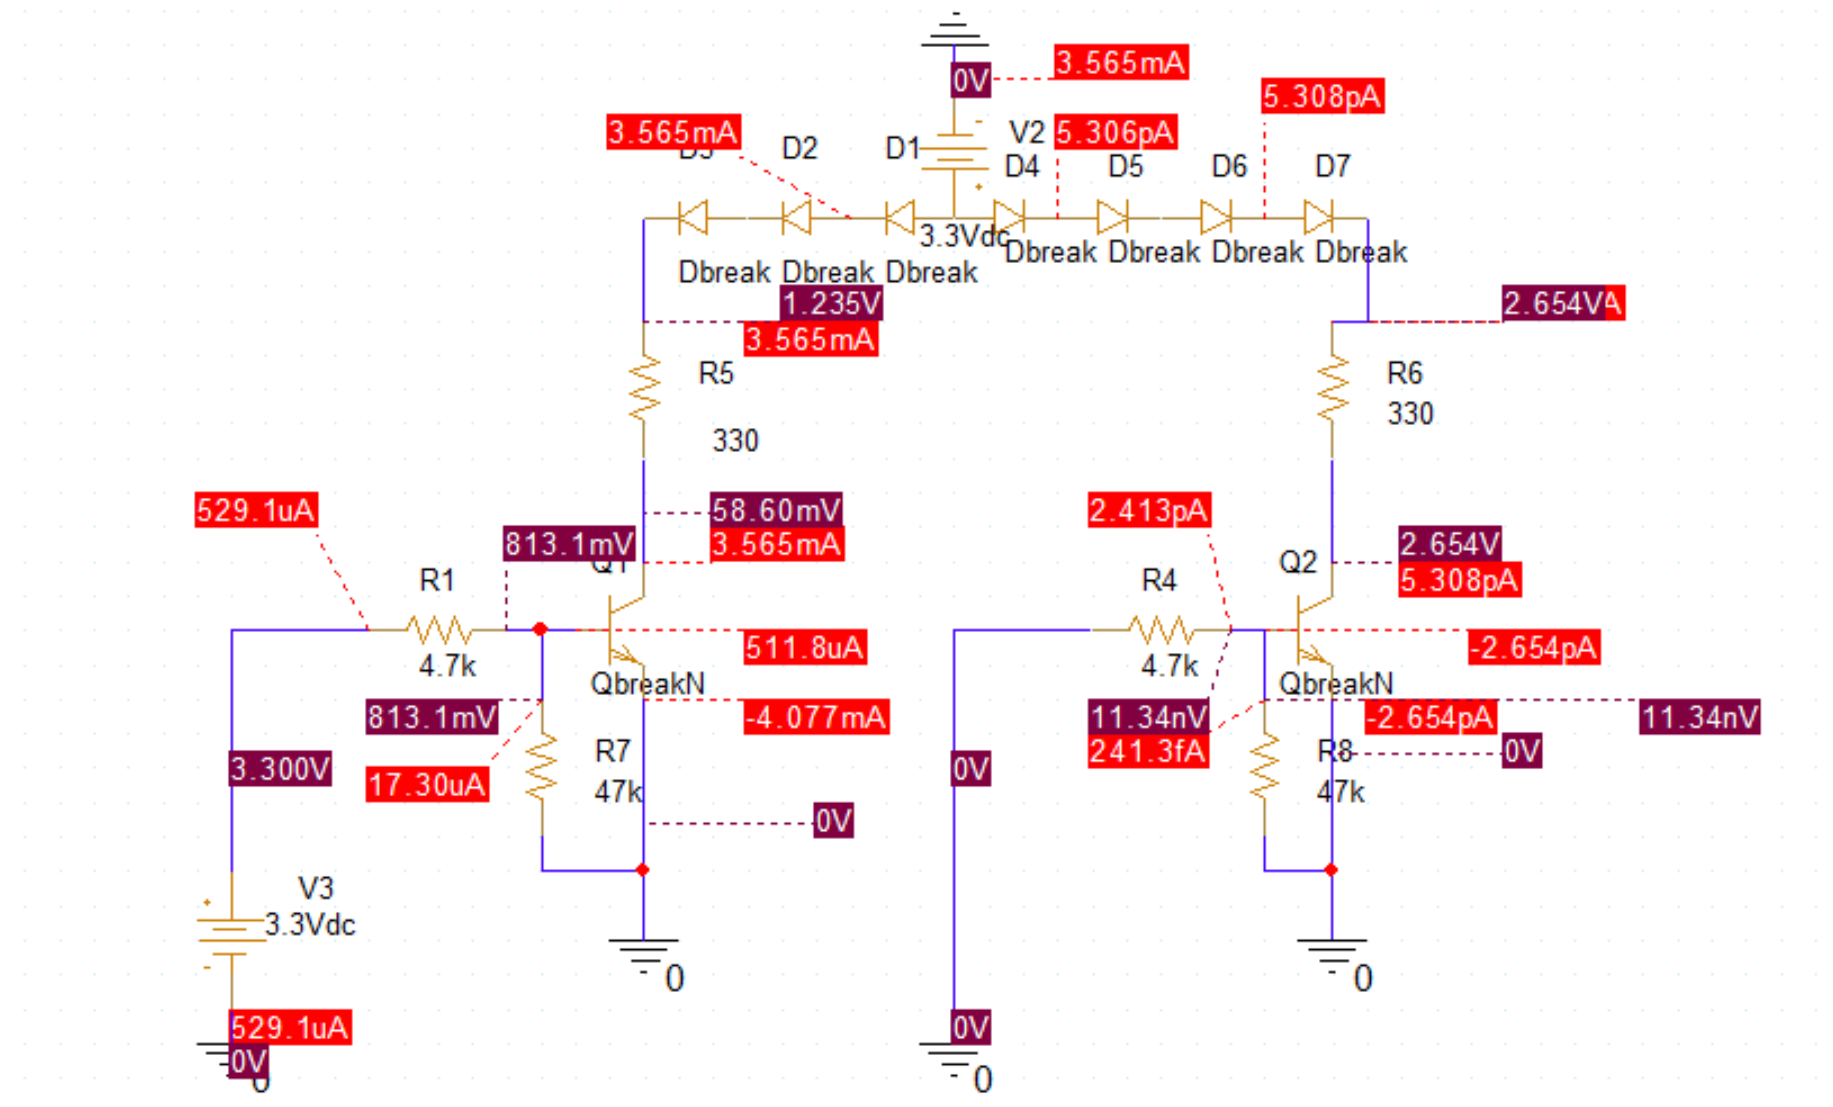
\includegraphics[width=0.95\textwidth]{graphics/section4/f6.png}
    \caption{Simulation red led on and green led off}
\end{figure}

\pagebreak

\textbf{Nhận xét} Ta thấy khi cả 2 chân LED0 và LED1 tích cực, có dòng điện đi qua cả hai đèn chứng tỏ cả hai đèn đều sáng. Khi ta điều khiển chân LED0 tích cực mức cao (3.3V) và chân LED1 tích cực mức thấp (0V), thì chỉ có dòng điện qua đèn đỏ (đèn đỏ bật) còn dòng qua đèn xanh gần bằng 0 (đèn xanh tắt). Điều này cho thấy 2 chân LED0 và LED1 điều khiển 2 đèn thông qua transitor BJT NPN.
